\begin{figure}
	\centering
	\pgfplotsset{every axis legend/.append style={
		at={(1.05,0.5)},
		anchor=west}}
	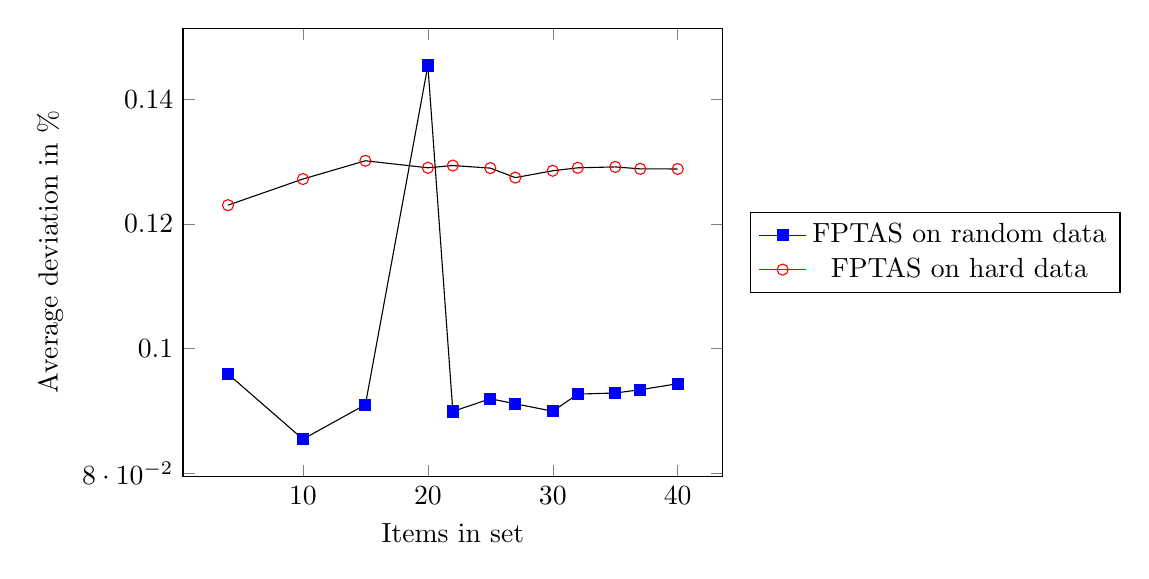
\begin{tikzpicture}
		\begin{axis}[
			xlabel=Items in set,
			ylabel=Average deviation in \%,
			scatter/classes={
				fptasN={mark=square*,blue},
				fptasH={mark=o,red}
				}
			]
			\addplot[scatter,%
				scatter src=explicit symbolic]%
			table[meta=label] {
                x y label
                4 .095931 fptasN
                10 .085455 fptasN
                15 .091002 fptasN
                20 .145440 fptasN
                22 .089912 fptasN
                25 .091948 fptasN
                27 .091139 fptasN
                30 .089941 fptasN
                32 .092691 fptasN
                35 .092870 fptasN
                37 .093395 fptasN
                40 .094362 fptasN
			};
			\addplot[scatter,%
				scatter src=explicit symbolic]%
			table[meta=label] {
				x y label
				4 .123029 fptasH
                10 .127224 fptasH
                15 .130156 fptasH
                20 .129032 fptasH
                22 .129395 fptasH
                25 .128979 fptasH
                27 .127454 fptasH
                30 .128554 fptasH
                32 .129028 fptasH
                35 .129171 fptasH
                37 .128856 fptasH
                40 .128841 fptasH
			};
			\addlegendentry{FPTAS on random data}
			\addlegendentry{FPTAS on hard data}
		\end{axis}
	\end{tikzpicture}
\caption{Average deviation in FPTAS algorithm}
\label{plot:deviation2}
\end{figure}
